\documentclass[11pt]{article}
\usepackage[final]{acl}
\usepackage{times}
\usepackage{latexsym}
\usepackage[T1]{fontenc}
\usepackage[utf8]{inputenc}
\usepackage{microtype}
\IfFileExists{inconsolata.sty}{\usepackage{inconsolata}}{}
\usepackage{graphicx}
\usepackage{booktabs}
\usepackage{multirow}
\usepackage{amsmath,amssymb}
\usepackage{xcolor}
\usepackage{tcolorbox}
\newcommand{\todo}[1]{\textcolor{red}{[TODO: #1]}}

\title{Replicating DetectGPT and Testing it on Machine-Generated Student Essays}

\author{Bimarsh Khatri \\
  Student ID 49140124 \\
  COMP8240 Applications of Data Science, Macquarie University}

\begin{document}
\maketitle

\begin{abstract}
DetectGPT \citep{mitchell2023detectgpt} flags a passage as machine-written when small rewrites of it consistently lower a language model's log-probability. We replicate the method with the authors' code on the original datasets, using the paper's GPT-2 XL configuration on a single 8\,GB laptop GPU, and show which settings explain the gap between our earlier pilot runs and the published numbers. We then test the method on student writing: two existing datasets (Kaggle LLM-Detect and HC3) and a new dataset of 600 student/LLM essay pairs built from the PERSUADE 2.0 corpus with two open instruction-tuned generators. Finally we compare DetectGPT with two LLM judges. On XSum and SQuAD DetectGPT reaches AUROC 0.96, close to the paper's 0.99 and above every zero-shot baseline. On the new essays it reaches 0.98 while the supervised RoBERTa detector falls to chance, and, unlike the likelihood baselines, it does not depend on the human essays being poorly written. \todo{judge headline}
\end{abstract}

%=====================================================================
\section{Introduction}
Universities now have to decide whether an essay was written by a student or by a chatbot, and the detectors on offer are mostly closed and untested on student writing. DetectGPT is attractive here because it is \emph{zero-shot}: it needs no labelled training data, only the token probabilities of a language model.

The project had three goals: (1) reproduce DetectGPT's results with the original code on the original data, (2) measure how well it carries over to student essays, including a newly constructed dataset, and (3) compare it with LLMs used as judges. Along the way it uses several of the unit's techniques: running published research code in an isolated Python environment, scripts that gather data from the Internet (Hugging Face, Kaggle, GitHub), data cleaning and normalisation, generating new data with LLMs, LLM-as-judge evaluation, statistical analysis (bootstrap intervals, Cohen's $\kappa$), and reproducible reporting with \LaTeX{} and GitHub. Code, the new dataset and all result files are public.\footnote{\url{https://github.com/BimarshKhatri123/dectect-gpt-replication}}

%=====================================================================
\section{The Paper and Why it was Chosen}
\label{sec:paper}
\paragraph{Summary.} \citet{mitchell2023detectgpt}\footnote{\url{https://proceedings.mlr.press/v202/mitchell23a.html}} observe that text sampled from a model $p_\theta$ tends to sit in a region of \emph{negative curvature} of $\log p_\theta$: almost any small rewrite of a machine-generated passage lowers its log-probability, whereas rewrites of human text may raise or lower it. DetectGPT turns this into the \emph{perturbation discrepancy}
\begin{equation}
d(x) = \log p_\theta(x) - \mathbb{E}_{\tilde{x}\sim q(\cdot\mid x)}\left[\log p_\theta(\tilde{x})\right],
\end{equation}
where $q$ masks 2-word spans covering 15\% of the words and refills them with T5 \citep{raffel2020t5}. The expectation is estimated from $k$ perturbations, and the paper's Algorithm~1 thresholds the normalised score $d(x)/\tilde\sigma_x$ (the ``z'' variant). Through the Hutchinson trace estimator \citep{hutchinson1989stochastic} the authors relate $d(x)$ to the trace of the Hessian of $\log p_\theta$. Nothing is trained; the scoring model only has to expose token log-probabilities.

\paragraph{Evaluation framework.} Each experiment uses $n$ human passages and $n$ machine passages generated by prompting the source model with the first 30 tokens of each human passage (temperature-1 sampling); both texts in a pair are cut to the same length. Performance is AUROC, the probability that a random machine passage scores higher than a random human one. DetectGPT is compared with four zero-shot statistics from the same model, namely average log-likelihood $\log p(x)$, average token rank, average log-rank \citep{gehrmann2019gltr} and predictive entropy, and with two supervised detectors (RoBERTa-base/large fine-tuned on GPT-2 output; \citealp{solaiman2019release}).

\paragraph{Reported results.} In the paper's Table~1 (500 pairs per dataset) DetectGPT is the best zero-shot method in 14 of 15 dataset/model combinations, averaging AUROC 0.97 on XSum, 0.92 on SQuAD and 0.97 on WritingPrompts. For the GPT-2 (1.5B) source model, the column we replicate, it scores 0.99 on all three datasets, against 0.89/0.94/0.98 for LogRank, the strongest baseline. The supervised detectors match DetectGPT on news-like text but drop sharply under domain shift (PubMedQA, German WMT16).

\paragraph{Justification.} The paper was published at ICML 2023, which CORE ranks A* and which is among the highest-ranked AI venues by Google Scholar h5-index, and it has been cited over \todo{N} times (Google Scholar, November 2026). It became the reference point for zero-shot detection, with direct successors such as Fast-DetectGPT \citep{bao2024fast} and Binoculars \citep{hans2024binoculars}. It is also well suited to replication: code, run scripts and datasets are public, and with no training step any difference in results can be traced to a few settings (scoring model, mask-filling model, number of perturbations). Finally, the paper never tests student writing, which is the setting where detectors are actually used.

%=====================================================================
\section{The Original Datasets}
\label{sec:origdata}
The paper uses \textbf{six datasets from five sources} (WMT16 contributes an English and a German set). In every case the human passages come from the dataset and the machine passages are generated from the first 30 tokens of each human passage.
\begin{itemize}\itemsep0pt
\item \textbf{XSum}\footnote{\url{https://huggingface.co/datasets/EdinburghNLP/xsum}} \citep{narayan2018xsum}: BBC news articles (field \texttt{document}), standing in for fake news.
\item \textbf{SQuAD}\footnote{\url{https://huggingface.co/datasets/rajpurkar/squad}} \citep{rajpurkar2016squad}: Wikipedia paragraphs (field \texttt{context}), the paper's proxy for machine-written academic essays.
\item \textbf{WritingPrompts}\footnote{\url{https://www.kaggle.com/datasets/ratthachat/writing-prompts}} \citep{fan2018hierarchical}: Reddit prompt/story pairs stored as two line-aligned files (\texttt{valid.wp\_source}, \texttt{valid.wp\_target}) with \texttt{<newline>} markers; creative writing.
\item \textbf{PubMedQA}\footnote{\url{https://huggingface.co/datasets/qiaojin/PubMedQA}} \citep{jin2019pubmedqa}: 1{,}000 expert-labelled biomedical questions (\texttt{pqa\_labeled}); the human text is ``\texttt{Question: q Answer: a}'' and the model is prompted with the question only.
\item \textbf{WMT16 English} and \textbf{German}\footnote{\url{https://huggingface.co/datasets/wmt16}} \citep{bojar2016wmt}: one side of the de--en news translation corpus, keeping documents of 100--150 words.
\end{itemize}
XSum, SQuAD and WritingPrompts form the main comparison (paper Table~1); PubMedQA and WMT16 test domain and language shift (paper Fig.~4 and Table~2). The code removes duplicates and newlines, keeps passages over 250 words for the first three datasets, and drops anything longer than 512 T5 tokens. Figure~\ref{fig:snippets} shows an XSum pair.

\begin{figure}[t]
\small
\begin{tcolorbox}[colback=gray!5,colframe=gray!50,boxsep=1pt,left=2pt,right=2pt,top=1pt,bottom=1pt]
\textbf{XSum, human:} \todo{xsum human snippet}\\[3pt]
\textbf{XSum, GPT-2 XL from the first 30 tokens:} \todo{xsum machine snippet}\\[3pt]
\hrule\vspace{3pt}
\textbf{New data, student (score 2/6):} \emph{``Advantages of limiting car ussage is if citizens limit their car usage there will be cut on greenhouse gas emissions, lower stress levels, and improve safety. Limiting car ussage will help reduces greenhouse gases\ldots''}\\[3pt]
\textbf{New data, Qwen2.5-1.5B, same prompt:} \emph{``Limiting car usage offers numerous advantages that go beyond reducing carbon footprints. By encouraging alternatives like biking, walking, or public transit, societies can significantly decrease congestion\ldots''}
\end{tcolorbox}
\caption{Opening words of a human/machine pair from the original XSum data and from our new PERSUADE-based dataset (``Car-free cities'' prompt).}
\label{fig:snippets}
\end{figure}

%=====================================================================
\section{Replication of the Original Work}
\label{sec:replication}
\paragraph{Environment.} We ran the authors' repository\footnote{\url{https://github.com/eric-mitchell/detect-gpt}} on a Windows~11 laptop with an RTX~4060 Laptop GPU (8\,GB), 16\,GB RAM, Python~3.10, PyTorch~2.13 (CUDA~12.6), Transformers~4.44.2 and Datasets~2.14.7. Getting it to run needed a few fixes, all marked \texttt{NEW} in \texttt{run.py}: WritingPrompts must be read as UTF-8 (Windows defaults to cp1252 and crashes), result folder names must not contain ``\texttt{:}'', and a Hugging Face cache copied between folders silently broke its symbolic links (tokenizer files became 52-byte text stubs). Every run is launched by \texttt{experiments/run\_suite.py}, which logs the exact command line and run time; all scripts used for the replication, with our changes to the original code marked, are in our public repository.\footnote{\url{https://github.com/BimarshKhatri123/dectect-gpt-replication} (replication: \texttt{run.py}, \texttt{experiments/}; setup: \texttt{README.md}, \texttt{requirements.txt}).}

\paragraph{Configuration.} We replicate the GPT-2 column of the paper's Table~1: GPT-2 XL (1.5B) as source and scoring model, 2-word spans and \texttt{pct\_words\_masked}=0.3 (the code masks $0.3\times\frac{2}{2+2}=15\%$ of words once the one-word buffer around each span is counted, matching the paper), and $k\in\{1,10,100\}$. Two departures were forced by the hardware. (i) The paper fills masks with T5-3B; on our 8\,GB GPU T5-3B spilled into system RAM and took about 9\,s per perturbed text, so a run would take days. We use T5-large, the mask filler the paper itself uses for its perturbation-count study (Fig.~8). (ii) We use $n=200$ pairs instead of 500 and report 95\% bootstrap confidence intervals. (iii) For WMT16 English and German the authors' script uses the multilingual mGPT (1.3B) scoring model with an mT5-XL (3.7B) mask filler; we keep mGPT and use mT5-large (1.2B), the same kind of substitution as T5-large for T5-3B. To fit the budget we also added speed options that leave the method unchanged: GPT-2 XL runs in fp16, perturbed texts are scored in batches of 8 (checked at run time against one-at-a-time scores; maximum difference $8\times10^{-4}$), the $k=1$ and $k=10$ estimates reuse the first $k$ of the 100 perturbations, and perturbations are cached per text so an interrupted run resumes. A 200-pair run on new texts takes about 3.4\,h.

\begin{table}[t]
\centering\small
\setlength{\tabcolsep}{3.5pt}
\begin{tabular}{lcccccc}
\toprule
 & \multicolumn{2}{c}{XSum} & \multicolumn{2}{c}{SQuAD} & \multicolumn{2}{c}{WritingPr.} \\
Method & ours & paper & ours & paper & ours & paper \\
\midrule
$\log p(x)$ & 0.89 & 0.86 & 0.90 & 0.91 & \todo{} & 0.97 \\
Rank        & 0.80 & 0.79 & 0.84 & 0.83 & \todo{} & 0.87 \\
LogRank     & 0.91 & 0.89 & 0.94 & 0.94 & \todo{} & 0.98 \\
Entropy     & 0.55 & 0.60 & 0.59 & 0.58 & \todo{} & 0.37 \\
DetectGPT   & \textbf{0.96} & \textbf{0.99} & \textbf{0.95} & \textbf{0.99} & \todo{} & \textbf{0.99} \\
\quad 95\% CI & \multicolumn{2}{l}{[.94, .98]} & \multicolumn{2}{l}{[.93, .97]} & \multicolumn{2}{l}{[\todo{}]}\\
\midrule
RoBERTa-base  & 0.98 & -- & 0.96 & -- & \todo{} & -- \\
RoBERTa-large & 1.00 & -- & 0.99 & -- & \todo{} & -- \\
\bottomrule
\end{tabular}
\caption{Replication of the GPT-2 column of Table~1 in \citet{mitchell2023detectgpt}: AUROC, GPT-2 XL source/scoring model, $k=100$, $n=200$ (paper: $n=500$, T5-3B). DetectGPT is the z-normalised variant.}
\label{tab:replication}
\end{table}

\paragraph{Results.} Table~\ref{tab:replication} compares our numbers with the paper. \todo{final sentence per dataset}. On XSum DetectGPT reaches 0.961 (the unnormalised $d$ variant 0.954), above the best zero-shot baseline LogRank (0.912), so the paper's main claim reproduces: DetectGPT beats every statistic computed from the same model. The baselines themselves match the paper closely: $\log p(x)$ 0.89 vs 0.86, LogRank 0.91 vs 0.89, Entropy 0.55 vs 0.60. The 100-pair run gave 0.965, so the estimate is stable in $n$. SQuAD gives the same picture: DetectGPT 0.952 [0.931, 0.969] against LogRank 0.938, with every baseline within 0.01 of the paper. \todo{WP/PubMed/WMT sentence}. As in the paper, the supervised RoBERTa detectors do very well on GPT-2 news text, which is the domain they were trained on.

\paragraph{How close, and why not closer.} DetectGPT lands about 0.02--0.03 below the paper on every dataset, while the baselines, which use no perturbations, match the paper to within about 0.03 in either direction. The gap is therefore in the perturbation step, and the evidence points to the smaller mask-filling model. (i) The paper's Fig.~7 shows AUROC rising with mask-filler size, and our ablation (Fig.~\ref{fig:pert}, bottom) shows the same trend from T5-small to T5-large. \todo{ablation numbers}. (ii) The number of perturbations matters a lot: on XSum AUROC rises from 0.77 ($k=1$) to 0.89 ($k=10$) and 0.96 ($k=100$), the same shape as the paper's Fig.~8. This also explains our pilot runs (Assignments 1--2), which used T5-small and $k=10$ and found DetectGPT \emph{below} LogRank on PubMedQA (0.79 vs 0.86); with the paper's settings the order is restored. (iii) With $n=200$ the 95\% intervals are about $\pm0.02$, so part of the remaining gap is sampling noise. We found no sign of an error in the original work; the shortfall is what the paper's own ablations predict for a smaller mask filler.

\paragraph{Where the method works and where it fails.} Looking at individual XSum errors (GPT-2 XL, $k=100$) shows a pattern. The human articles with the \emph{highest} DetectGPT scores are formulaic wire-style reports, for example an ONS labour-market release (``Unemployment fell to 1.69 million between January and March, down 2,000 from the previous quarter. The jobless rate remained at 5.1\%\ldots''). Such text is so predictable that almost any rewrite lowers its probability, just as for machine text. The machine passages DetectGPT \emph{misses} are GPT-2 continuations that drift into implausible content (an art broker who ``did not approve of nudity'' promoting a nude painting). They already have low log-probability ($-2.99$ per token, against a median of $-2.19$ for machine passages), so rewrites cannot lower it much. DetectGPT therefore detects text that is \emph{typical} for the model; fluent but formulaic human prose is its main source of false positives. We also checked the paper's suggestion (Fig.~9) that a threshold of about $d=0.1$ separates the classes across domains. On XSum half of the human articles exceed 0.1 (median 0.10, machine 0.21), so the ranking is good but this fixed threshold does not transfer to our setup (Section~\ref{sec:results} shows the same on student essays).

\begin{figure}[t]
\centering
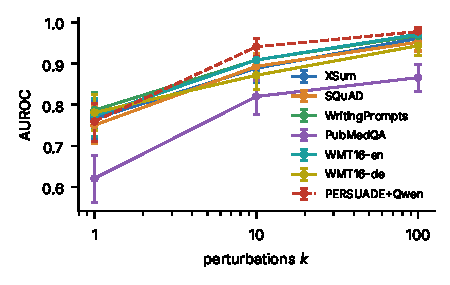
\includegraphics[width=\columnwidth]{figures/fig_perturbations.pdf}\\[2pt]
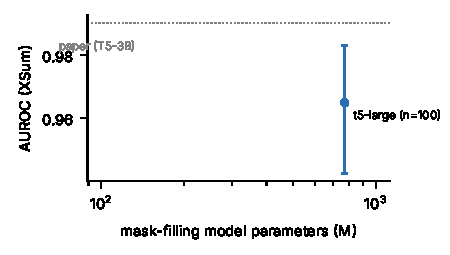
\includegraphics[width=\columnwidth]{figures/fig_mask_ablation.pdf}
\caption{Top: DetectGPT (z) AUROC against the number of perturbations $k$. Bottom: XSum AUROC ($k=100$) by mask-filling model. Error bars are 95\% bootstrap intervals.}
\label{fig:pert}
\end{figure}

%=====================================================================
\section{Construction of New Data}
\label{sec:newdata}
The extension asks whether DetectGPT works on \emph{student essays}, where a false accusation is costly. We use two existing datasets and one we built (Table~\ref{tab:newdata}).

\paragraph{Existing dataset 1: Kaggle LLM-Detect.}\footnote{\url{https://www.kaggle.com/competitions/llm-detect-ai-generated-text}} The training file of this competition \citep{king2023kaggle} has 1{,}378 essays by US students in grades 6--12 on two prompts (``Car-free cities'', ``Does the electoral college work?''), but only three are machine-written. We therefore keep the 1{,}375 human essays, cut each to its first 250 words, and generate the machine side exactly as the paper does (GPT-2 XL continuing the first 30 tokens). This tests the original protocol on a new domain.

\paragraph{Existing dataset 2: HC3.}\footnote{\url{https://huggingface.co/datasets/Hello-SimpleAI/HC3}} HC3 \citep{guo2023hc3} pairs human answers with ChatGPT answers to the same question in five domains (computer-science Wikipedia, open QA, finance, medicine, Reddit ELI5). It tests the \emph{black-box} case: ChatGPT's probabilities are unavailable, so GPT-2 XL acts as a surrogate scorer. For every question we take the first human and first ChatGPT answer of at least 100 words, drop ChatGPT refusals (``As an AI\ldots''), and cut both to the same length ($\le$250 words). Human answers from Reddit and WikiQA contain tokenisation artefacts (`` ,'', ``( '') that LLM output never has, which would give the game away, so the same normaliser is applied to both sides. Of 24{,}322 questions, 14{,}171 yield a usable pair; we keep up to 200 per domain, interleaved so any prefix is domain-balanced. Open-QA human answers are short (WikiQA sentences), so that domain contributes only 10 of the 810 pairs.

\paragraph{Constructed dataset: PERSUADE essay pairs.} Our proposal planned roughly 30 assignment prompts with paired human/LLM answers; the pilot in Assignment~2 had only 2 prompts and 90 machine essays, and the marker asked for larger datasets and more detail on construction. The final dataset is built in four scripted steps (\texttt{new\_data/}):
\begin{enumerate}\itemsep0pt
\item \textbf{Prompts.} PERSUADE 2.0 \citep{crossley2024persuade} contains 15{,}594 argumentative essays by US students in grades 6--12 on 15 prompts, each with an expert holistic score from 1 to 6. We keep the eight \emph{independent} prompts and the two \emph{text-dependent} prompts whose source articles we have (from the Kaggle prompt file). The other five text-dependent prompts are excluded: their source articles are not distributed, so an LLM would have to invent the article content, giving the machine essays a systematic difference that has nothing to do with authorship.
\item \textbf{Human essays.} For each prompt we sample 60 essays of at least 150 words (seed 0), keeping the essay id, holistic score and grade, but \emph{not} the demographic fields (gender, race/ethnicity, ELL, disability, economic status).
\item \textbf{Machine essays.} Two open instruction-tuned models from different families, Qwen2.5-1.5B-Instruct \citep{qwen2025qwen25} and SmolLM2-1.7B-Instruct \citep{allal2025smollm2}, each write 30 essays per prompt (temperature 0.8, top-$p$ 0.95, fp16, seed 0). Each model receives the \emph{same assignment text the students saw}, the source passages for text-dependent prompts, and the persona ``a US student in grade $g$'', where $g$ is the grade of the students who wrote that prompt; it is asked for about 400 words of plain paragraphs. Markdown, title lines and placeholders such as ``[Your Name]'' are removed, and outputs under 150 words are discarded; over 96\% of generations passed.
\item \textbf{Pairing.} Each machine essay is paired with a \emph{different} student essay on the same prompt (the two generators get disjoint halves of the 60), both sides are cut to the same length ($\le$250 words, mean 242), and prompts are interleaved.
\end{enumerate}
The result is 600 pairs (1{,}200 texts) over 10 prompts, released as one long-format CSV with provenance for every text (source id, generator, decoding settings, expert score for human essays). Matching the length of each pair removes the most obvious shortcut; the remaining difference between the classes is \emph{register}. Student essays contain spelling and grammar errors, while the LLM essays are fluent and generic (Fig.~\ref{fig:snippets}). Because PERSUADE comes with expert scores, we can test directly whether a detector is merely spotting weak writing (Section~\ref{sec:results}).

\begin{table}[t]
\centering\small
\setlength{\tabcolsep}{3pt}
\begin{tabular}{lrrl}
\toprule
Dataset & pairs & words & machine text \\
\midrule
Kaggle LLM-Detect & 1{,}375 & \todo{} & GPT-2 XL (white-box) \\
HC3 & 810 & 158 & ChatGPT (black-box) \\
PERSUADE + Qwen & 300 & 242 & Qwen2.5-1.5B-Inst. \\
PERSUADE + SmolLM2 & 300 & 242 & SmolLM2-1.7B-Inst. \\
\bottomrule
\end{tabular}
\caption{New datasets. ``Pairs'' is the number available; each experiment uses the first 200. ``Words'' is the mean length after pairing and truncation.}
\label{tab:newdata}
\end{table}

\paragraph{Annotation and agreement.} The labels come from construction, so no annotation is needed to create the data. Annotation enters at two points. First, the expert holistic scores shipped with PERSUADE act as gold quality labels for the human essays. Second, two LLM judges from different model families score every text (Section~\ref{sec:results}), and we report their agreement with each other (Cohen's $\kappa$) and, for quality, with the expert scores (quadratic weighted $\kappa$). \todo{human annotation of 40 blind items if done}.

%=====================================================================
\section{Results on New Data}
\label{sec:results}
All new-data runs use the replication configuration (GPT-2 XL scorer, T5-large, $k=100$, $n=200$). Where the machine text was not written by GPT-2 XL, GPT-2 XL acts as a surrogate scorer; for the two PERSUADE subsets we also score with the generator itself (\emph{white-box}), reusing the same cached perturbations. Table~\ref{tab:newresults} gives the results.

\begin{table*}[t]
\centering\small
\begin{tabular}{lcccccc}
\toprule
 & Kaggle & HC3 & \multicolumn{2}{c}{PERSUADE + Qwen} & \multicolumn{2}{c}{PERSUADE + SmolLM2} \\
Scoring model & GPT-2 XL & GPT-2 XL & GPT-2 XL & Qwen (white-box) & GPT-2 XL & SmolLM2 (white-box) \\
\midrule
$\log p(x)$  & \todo{} & \todo{} & 0.82 & \todo{} & \todo{} & \todo{} \\
Rank         & \todo{} & \todo{} & 0.86 & \todo{} & \todo{} & \todo{} \\
LogRank      & \todo{} & \todo{} & 0.80 & \todo{} & \todo{} & \todo{} \\
Entropy      & \todo{} & \todo{} & 0.21 & \todo{} & \todo{} & \todo{} \\
DetectGPT ($k=100$) & \todo{} & \todo{} & \textbf{0.98} & \todo{} & \todo{} & \todo{} \\
\midrule
RoBERTa-base  & \todo{} & \todo{} & 0.50 & -- & \todo{} & -- \\
RoBERTa-large & \todo{} & \todo{} & 0.51 & -- & \todo{} & -- \\
LLM judge: Qwen2.5-3B & -- & 0.42 & \multicolumn{2}{c}{0.30} & \multicolumn{2}{c}{0.36} \\
LLM judge: Phi-3.5-mini & -- & 0.39 & \multicolumn{2}{c}{0.33} & \multicolumn{2}{c}{0.31} \\
\bottomrule
\end{tabular}
\caption{AUROC on the new data ($n=200$ pairs each). The supervised and LLM-judge detectors do not use a scoring model. Replication numbers for comparison: DetectGPT 0.96 on XSum.}
\label{tab:newresults}
\end{table*}

\paragraph{DetectGPT on student essays.} On the PERSUADE + Qwen essays DetectGPT reaches 0.978, \emph{higher} than on any replication dataset, even though GPT-2 XL did not write these essays. The zero-shot baselines lose much more ground (LogRank 0.80 vs 0.91 on XSum), and the supervised RoBERTa detectors, which are near-perfect on GPT-2 news, fall to chance (0.50/0.51). This is the paper's domain-shift result in a sharper form: a detector trained on one generator's output does not carry over to a modern instruction-tuned model writing in a different genre, while the curvature test does. \todo{SmolLM2, white-box vs surrogate, Kaggle, HC3}.

\paragraph{Is it just spotting weak writing?} Student essays have spelling and grammar errors that make them less probable under any language model, so a high AUROC could simply mean that poor writing is easy to tell apart from fluent text. The expert scores let us test this (Fig.~\ref{fig:quality}): we compare all 200 machine essays with only the weakest human essays (score $\le$2, $n=42$) or only the strongest (score $\ge$4, $n=99$). LogRank falls from 0.94 to 0.75 and $\log p(x)$ from 0.96 to 0.77, so these baselines mostly separate \emph{poor} writing from machine text. DetectGPT stays at 1.00 and 0.97. Because it compares a text with rewrites of itself, a fluent student essay is not flagged just for being fluent, and that is the property that matters most for academic integrity.

\begin{figure}[t]
\centering
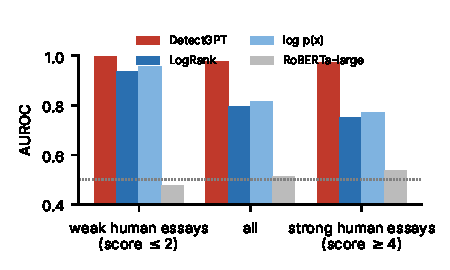
\includegraphics[width=\columnwidth]{figures/fig_quality.pdf}
\caption{PERSUADE + Qwen, GPT-2 XL scorer: AUROC of all 200 machine essays against weak, all, or strong human essays (expert holistic score).}
\label{fig:quality}
\end{figure}

\paragraph{Error analysis.} The student essays DetectGPT most wrongly flags are the most polished ones: formal letters that follow a textbook argumentative template (``Dear state senator, Many people believe that the Electoral College should be abolished, while others believe\ldots''). The machine essays it misses either adopt a student persona (``As a ninth grader who values both technology and education equally\ldots'') or use unusually ornate vocabulary (``The advent of smart planning across continents highlights a pivotal shift towards non-car-centric lifestyles\ldots''), which GPT-2 XL finds improbable from the start. The raw discrepancy also shifts between domains: the median $d$ is 0.005 for student essays and 0.076 for Qwen essays, so the paper's threshold of 0.1 would catch only 15\% of machine essays here, against all of them on XSum. A deployed detector would need a threshold calibrated on the target population.

\paragraph{Operating point.} AUROC hides how many students would be falsely accused. Fixing the false-positive rate at 1\%, DetectGPT catches 73\% of the Qwen essays (86\% at 5\%), LogRank 3\% and RoBERTa-large none. On XSum, DetectGPT catches 56\% at 1\%.

\paragraph{LLM-as-judge.} The judges play two roles. As \emph{detectors} they answer a two-option question (human or AI) about each text; we read the probability of each answer letter and average over both answer orders to cancel letter bias, which gives a continuous score comparable with DetectGPT by AUROC on the same pairs. As \emph{quality raters} they score every essay from 1 to 6 on the PERSUADE scale, which can be checked against the expert scores and shows whether the constructed essays are on-task.

As detectors both judges fail, and in an informative way (Table~\ref{tab:newresults}). Their AUROC is \emph{below} 0.5 on every dataset (0.30--0.42): after averaging out letter bias, they consider the LLM essays slightly \emph{more} human than the student essays. The raw answers are dominated by answer position. Qwen2.5-3B picks option ``A'' about 97\% of the time whatever that option says; the two answer orders give the same decision for only 8--22\% of texts across judges and datasets, and the two judges agree only weakly with each other ($\kappa=0.16$--$0.30$). The weakest result, 0.30, is the Qwen judge on Qwen-written essays, consistent with reports that LLM evaluators favour text from their own model family \citep{panickssery2024self}. As quality raters the judges are far more consistent: they agree with each other (quadratic weighted $\kappa=0.73$), their scores correlate moderately with the expert holistic scores on the human essays (Spearman 0.26--0.47), and they rate the machine essays higher than the student essays (4.5--4.7 vs 3.5--3.7 out of 6). So the constructed machine essays are coherent and on-task, which supports the quality of the new data, but fluent text is exactly what these small judges take for human writing. In our setting an LLM judge is a usable quality rater and not a usable detector, while DetectGPT, which never sees a label, is both accurate and robust to writing quality.

\paragraph{How this relates to the replication.} Three differences from the replication protocol should be kept in mind. (i) In the replication the source and scoring model are the same (white-box); on HC3 and PERSUADE they are not, which the paper (Fig.~6) shows lowers AUROC, yet our surrogate scores stay high. (ii) The machine text here answers a prompt rather than continuing a 30-token prefix, so the two sides share a topic but not their opening words. (iii) Kaggle uses the paper's own protocol, so it isolates the change of domain from these other changes.

%=====================================================================
\section{Ethical Considerations}
\label{sec:ethics}
\paragraph{In the original paper.} The authors discuss misuse of detection (evasion by paraphrasing) and release their code and data openly, with the paper itself open access through PMLR and arXiv. Two issues get less attention. First, a detector's errors fall on people: \citet{liang2023biased} show that GPT detectors flag non-native English writing as machine-made far more often than native writing, so a high average AUROC can hide unfair treatment of a subgroup. Second, some source data were collected without the authors' consent for this use (Reddit stories in WritingPrompts; BBC articles in XSum), which is common practice but sits uneasily with the principle of respect.

\paragraph{If we published on the new data.} Under the \textit{Australian Code for the Responsible Conduct of Research} \citep{nhmrc2018code}, the relevant principles are honesty, rigour, transparency, fairness, respect and accountability.
\emph{Human data.} PERSUADE essays were written by school students, many of them minors. They were collected with consent by the corpus creators, released de-identified under CC BY-NC-SA 4.0, and we use them only for non-commercial research. Our release keeps the licence and attribution, and we deliberately leave out all demographic fields (data minimisation). Using existing, non-identifiable data is normally negligible-risk research under the \textit{National Statement} \citep{nhmrc2023national}, but a publication would still need an ethics determination from the university's HREC. Kaggle's competition data may not be redistributed, so we publish the scripts that rebuild that part rather than the text. HC3 is released under CC BY-SA.
\emph{Fairness.} The most important open question is whether DetectGPT's false positives fall disproportionately on English-language learners or students with disabilities. PERSUADE records these attributes, so the question can be answered, but only with ethics approval and care not to stigmatise those groups; we did not do this analysis here.
\emph{Harm from use.} Even at AUROC 0.98, a threshold that falsely flags 1 in 100 genuine essays still misses about a quarter of machine essays (Section~\ref{sec:results}), and over a cohort of thousands that is many false accusations. A detector score should therefore never be the sole evidence in a misconduct case. The LLM judges are worse still and not suitable for such decisions.
\emph{Transparency and open access.} All code, prompts, decoding settings, random seeds and per-run logs are public, and the generated essays are labelled as machine text so they cannot be passed off as student work. Both generators are released under the Apache-2.0 licence. Running every experiment took about \todo{N} GPU-hours on a laptop. Generative AI tools were used for coding assistance and drafting; all outputs were checked by the author, who takes responsibility for the content.

%=====================================================================
\section{Conclusions and Reflections}
\todo{after results}

\bibliography{references}

\appendix
\section{Reproducing the Results}
\label{app:repro}
All experiments are defined in \texttt{experiments/run\_suite.py}; the repository README lists the setup and the external downloads (WritingPrompts, Kaggle and PERSUADE cannot be redistributed in full).
{\small
\begin{verbatim}
pip install -r requirements.txt
python experiments/prefetch.py --cache_dir ../cache
python experiments/run_suite.py --suite all
python analysis/aggregate.py
\end{verbatim}}
\noindent A single replication run, for example XSum, is
{\small
\begin{verbatim}
python run.py --dataset xsum --dataset_key document
  --n_samples 200 --n_perturbation_list 1,10,100
  --base_model_name gpt2-xl
  --mask_filling_model_name t5-large
  --pct_words_masked 0.3 --span_length 2
  --base_half --ll_batch_size 8
  --reuse_perturbations
  --perturbation_cache perturbation_cache
\end{verbatim}}
\noindent Each run writes its arguments, predictions, AUROC/PR-AUC, ROC curves and run time to \texttt{results/final/<run>/}; \texttt{analysis/aggregate.py} computes the bootstrap intervals, TPR at fixed FPR, the quality-stratified AUROC, the judge tables and all figures from these files.

\section{Generation Prompt}
\label{app:prompt}
The machine essays for prompt ``Community service'' (grade 8) were generated from:
{\small
\begin{quote}\itshape
You are a US student in grade 8 completing a writing assignment. Task: Some of your friends perform community service. For example, some tutor elementary school children and others clean up litter. [\ldots] Write a letter to your principal in which you take a position on whether students should be required to perform community service. Support your position with examples. Write the essay now, about 400 words, as plain paragraphs. Do not include a title, headings, bullet points, placeholders such as [Your Name], or any commentary.
\end{quote}}
\noindent For text-dependent prompts the source passages are inserted before the task. The full prompt for every topic is printed by \texttt{python new\_data/make\_machine\_essays.py --print\_prompt <id>}.

\end{document}
